\documentclass[14pt]{extarticle}

\PassOptionsToPackage{backend=biber, style=gost-numeric, sorting=nty, language=auto}{biblatex}

\usepackage{imit_vkr}
\usepackage{graphicx}
\usepackage{amsmath}
\usepackage{amsfonts}
\usepackage{amssymb}
\usepackage{longtable}
\usepackage{array}
\usepackage{tikz}
\usepackage{pgfplots}

% Если hyperref не загружен в шаблоне, раскомментируйте:
% \usepackage{hyperref}

\addbibresource{literature.bib}

\begin{document}
   
%%%--------Титульная страница
%==Титульная страница
\thispagestyle{empty}
\begin{center}

\includegraphics[width=0.2\textwidth]{img/image.png}\\[0.5cm]

{\bf Министерство науки и высшего образования Российской Федерации}\\
Федеральное государственное бюджетное образовательное\\
учреждение высшего образования\\
{\bf <<Иркутский государственный университет>>}\\
(ФГБОУ ВО <<ИГУ>>)\\
{\bf Институт математики и информационных технологий}\\
Кафедра алгебраических и информационных систем\\
\end{center}

\vspace{1 cm}

\begin{center}
{\bf 
ОТЧЁТ ПО УЧЕБНОЙ ПРАКТИКЕ\\[1mm]
Научно-исследовательская работа \\[1mm]
(получение первичных навыков \\[1mm] 
научно-исследовательской работы)
}  

\end{center}

\vspace{2 cm}

{
\noindent\hbox to 0.48\textwidth {%	
	\mbox{ } \hfil} %
	\begin{tabular}[t]{l}
		Руководитель:\\ профессор кафедры алгебраических и\\
        информационных систем, д.ф.-м.н. \\
        Винокуров С.Ф.
		
	\end{tabular}		
}


\vspace{1.5cm}

{
\noindent\hbox to 0.48\textwidth {%
	\mbox{ } \hfil} %
	\begin{tabular}[t]{l}
		Студенты:\\
		Ашроев Евгений Вадимович\\
        Шилов Данил Иванович\\
        гр. 02371-ДБ, 3 курс ФИ

		
	\end{tabular}		
}


\vfill 
\noindent
\begin{minipage}{\textwidth}
\centering	 Иркутск 2026
\end{minipage}

%-------------
%Основная часть
%-------------

\mynonumbersection{Дневник прохождения учебной практики}

\begin{table}[h!]
\centering
\begin{tabular}{|p{2.5cm}|p{9cm}|p{3cm}|}
\hline
\textbf{Дата} & \textbf{Краткое содержание работы} & \textbf{Отметка о выполнении} \\
\hline
01.06.26 & Получение задания. Задача: поиск минимальной ДНФ недоопределенной булевой функции. Алгоритм: имитация отжига. & \\
\hline
02.06.26 --- 03.06.26 & Изучение теоретических основ алгоритма имитации отжига и модели термодинамического охлаждения. & \\
\hline
04.06.26 & Определение способов представления состояний булевой функции и адаптация операторов изменения конфигураций под АИО. & \\
\hline
05.06.26 --- 06.06.26 & Программная реализация логики алгоритма на Python и макетирование консольного TUI-интерфейса во фреймворке Textual. & \\
\hline
08.06.26 & Интеграция вычислительного модуля с интерфейсной оболочкой, отладка передачи данных через оперативную память. & \\
\hline
09.06.26 --- 10.06.26 & Тестирование работы алгоритма и подбор оптимального шага охлаждения системы. & \\
\hline
11.06.26 & Настройка вывода графиков зависимости целевой функции от итерации и скроллируемого лога векторов в терминале. & \\
\hline
13.06.26 & Сбор результатов экспериментов и оформление отчёта по исследовательской практике. & \\
\hline
\end{tabular}
\end{table}

\newpage

\mynonumbersection{ВВЕДЕНИЕ}

Поиск минимальной дизъюнктивной нормальной формы (ДНФ) недоопределенной булевой функции --- это классическая задача дискретной математики и логического проектирования. Она возникает при оптимизации топологии интегральных схем, минимизации логических цепей и автоматизации проектирования цифровых устройств, где требуется сократить количество логических элементов на кристалле. Задача относится к классу NP-трудных. С ростом числа переменных размерность пространства поиска растет экспоненциально, поэтому полный перебор конфигураций быстро становится нереализуемым. Но использование случайных эвристических подходов дает возможность находить качественные решения за вполне приемлемое время.

В данной работе разработано и исследовано программное приложение для оптимизации недоопределенных функций с помощью алгоритма имитации отжига. Этот метаэвристический метод концептуально повторяет термодинамический процесс постепенного охлаждения и кристаллизации металлов, при котором вещество переходит в состояние с минимальной внутренней энергией. Алгоритм моделирует это поведение за счет постепенного снижения расчетной температуры. На первых шагах программа допускает переход к ухудшающим состояниям с вероятностью $P = e^{-D/t_i}$, где $D$ --- разность энергий между состояниями. Это помогает вычислениям не застревать в локальных экстремумах, а затем, по мере остывания системы, сфокусироваться на поиске глобального минимума.

\newpage 

\section*{Постановка задачи}

Рассматривается классическая задача минимизации дизъюнктивной нормальной формы (ДНФ) булевой функции. У нас есть функция $f(x_1, x_2, \dots, x_n)$, заданная наборами своих значений. Нужно найти такую формулу в виде дизъюнкции элементарных конъюнкций, которая будет полностью эквивалентна этой функции, но получит минимальную сложность. А под сложностью здесь понимается суммарное число литералов во всех конъюнкциях выражения.

\[
\begin{gathered}
\text{Минимизировать } L(D) = \sum_{j=1}^{m} |K_j|, \\
\text{при ограничении } D(\chi) = f(\chi), \quad \forall \chi \in \text{dom}(f), \\
\text{где } D = K_1 \vee K_2 \vee \dots \vee K_m.
\end{gathered}
\]

Здесь $D$ --- это искомая дизъюнктивная форма, разбитая на $m$ отдельных конъюнкций $K_j$. Величина $|K_j|$ означает просто количество переменных, входящих в конкретную конъюнкцию, а $L(D)$ выражает итоговую сложность формулы. Наборы переменных $\chi$ берутся из области определения функции $\text{dom}(f)$.

\section*{Алгоритм имитации отжига}

Метод имитации отжига опирается на физическую модель, воспроизводящую поведение кристаллической решетки металла при нагреве и последующем медленном охлаждении \cite{skobcov}. Здесь любое состояние системы $S$ представляет собой конкретное решение задачи, а уровень внутренней энергии $E(S)$ выступает в качестве целевой функции, которую требуется минимизировать. Алгоритм начинает поиск с некоторого случайного варианта и высокой начальной температуры $T_0$.

На каждой итерации текущее состояние немного меняется на соседнее. Если энергия нового решения оказывается меньше, система переходит в него сразу. Но если новое состояние увеличивает энергию, переход все равно остается возможным. Вероятность $P$ такого шага рассчитывается по формуле:

\[
P = e^{-\frac{\Delta E}{T}},
\]

где $\Delta E$ --- разность энергий между новым и старым состояниями, а $T$ --- текущая температура. По ходу работы температура постепенно снижается. Из-за этого вероятность принять ухудшающее решение со временем падает, что помогает алгоритму сначала активно прыгать по разным локальным минимумам, а под конец стабилизироваться в оптимальной точке.

\section*{Описание задачи в терминах алгоритма}

В нашей задаче поиска минимальной ДНФ мы спроецировали физические понятия на математические. Состояние системы $S$ --- это текущая структура дизъюнктивной нормальной формы, которую мы кодируем вектором. Функция энергии $g$ отвечает за длину полученной формулы, то есть считает суммарное количество литералов. Чем формула короче, тем меньше у нее энергия. Функция изменения состояния $f$ берет текущий вектор и инвертирует в нем часть бит, смещая нас в соседнюю точку пространства поиска. А вероятность перехода в ухудшающее состояние вычисляется по классической формуле $P=e^{-D / t_i}$.

\section*{Параметры алгоритма}

Чтобы программу было удобно тестировать, все стартовые параметры мы вынесли в отдельный конфигурационный файл. Прямо из интерфейса пользователь задает начальную и конечную температуру, количество итераций на одном температурном срезе и весовые коэффициенты. В качестве закона изменения температуры мы добавили возможность выбрать один из трёх законов охлаждения: Линейный $t_i = t_{i-1} - \alpha$, Больцмона $t_i = t_0 \slash \ln(1+i)$ и Коши $t_i = t_0 \slash i$.

\section*{Реализация алгоритма и интерфейса программы}

Мы не стали запускать вычислительное ядро через сторонние процессы вроде \texttt{subprocess.run}, потому что это сильно тормозит работу. Вместо этого логика алгоритма напрямую импортируется в память интерфейса. Сами расчеты запускаются асинхронно через \texttt{asyncio.to\_thread}, поэтому консоль не зависает, пока процессор занят математикой.

Интерфейс подстраивается под окружение пользователя. Библиотека \texttt{darkdetect} \cite{darkdetect} при запуске опрашивает операционную систему и автоматически включает нужную тему --- светлую или темную. Если ОС не дает ответа, программа безопасно откатывается на нашу кастомную темную палитру.

\section*{Вычислительные эксперименты}

Для апробации мы сгенерировали несколько недоопределенных булевых функций. За ходом поиска можно следить прямо в терминале. Мы встроили графики, которые рисуются в консоли с помощью псевдографики. На экран в реальном времени выводится кривая зависимости энергии от номера текущей итерации. Ниже расположен скроллируемый лог истории сгенерированных векторов. Чтобы график строился корректно, вычислительный модуль на каждом шаге собирает значения энергии и температуры в отдельные списки и отдает их интерфейсу.

\begin{figure}[h!]
\centering
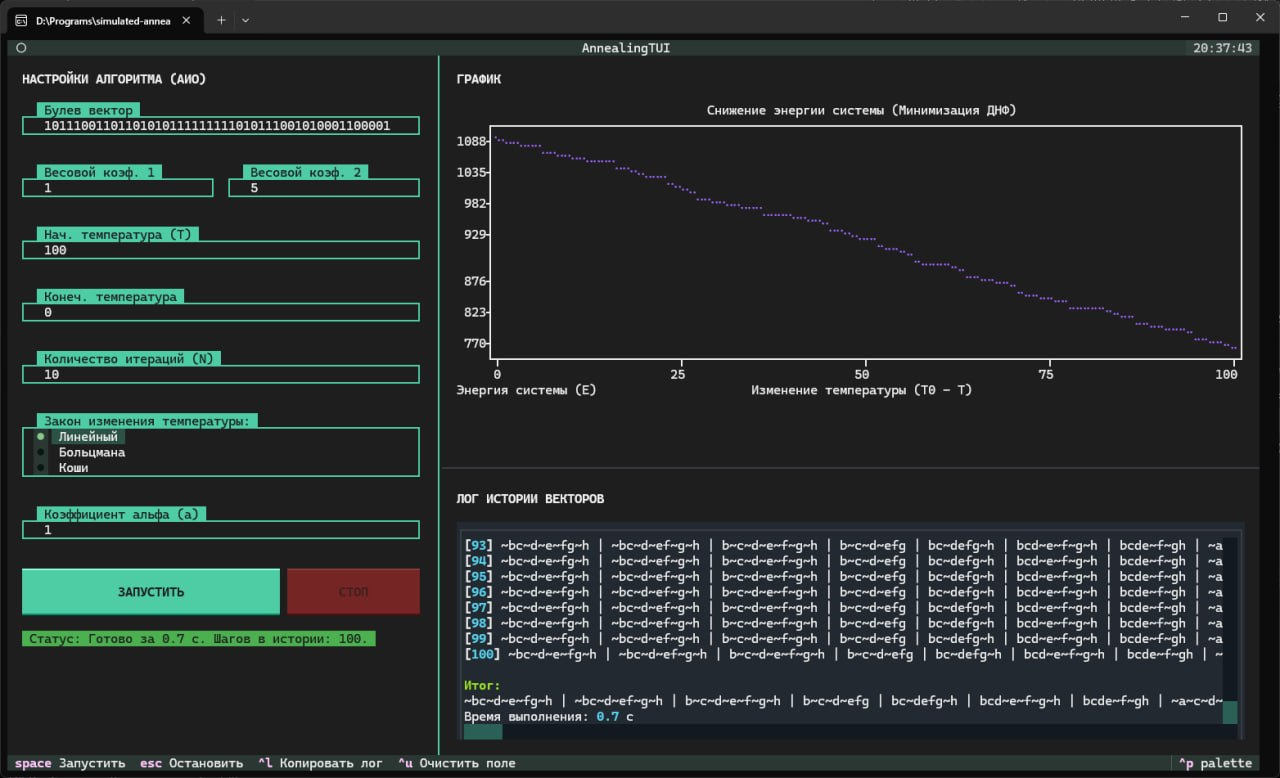
\includegraphics[width=0.95\textwidth]{img/screenshot_tui_main.jpg}
\caption{Интерфейс программы: график изменения энергии и лог сгенерированных векторов}
\label{fig:tui}
\end{figure}

Мы заметили, что если выставить слишком большой шаг $\alpha$, система остывает слишком быстро. Алгоритм не успевает перебрать достаточно состояний и застревает в локальных минимумах. А вот при небольшом и плавном шаге охлаждения результаты стабильно улучшаются, особенно на больших значениях начальной температуры.

\section*{Тестовые примеры}

Для проверки корректности работы алгоритма и тестирования производительности TUI-интерфейса мы использовали набор недоопределенных булевых функций различной размерности. Каждая функция кодировалась в виде бинарного вектора, где длина вектора определяет количество возможных входных наборов (от 4 до 64 значений).

Ниже представлены сгенерированные входные векторы, на которых проводилась отладка программы:

\begin{itemize}
    \item \texttt{10110011}
    \item \texttt{0110110100101101}
    \item \texttt{01000010110011101010110101011110}
    \item \texttt{0000001110011100011000011010010010111011011100110011100010001011}
    \item \texttt{...}
\end{itemize}

Все использованные вектора нецелесообразно вставлять в отчёт из-за их огромного размера. 

\section*{Итоги работы}

Приложение полностью решает поставленную задачу минимизации ДНФ. Модульная архитектура позволила вести разработку вычислительного ядра и интерфейса параллельно, а прямой импорт и асинхронное выполнение обеспечили высокую производительность и отзывчивость. В результате получился удобный консольный инструмент с графиками и автоматической сменой темы оформления.

\newpage

% Печать списка литературы (все цитированные источники)
\printbibliography[title={Список литературы}]

\end{document}